\chapter*{}

\begin{titlepage}
 
 
\setlength{\centeroffset}{-0.5\oddsidemargin}
\addtolength{\centeroffset}{0.5\evensidemargin}
\thispagestyle{empty}

\noindent\hspace*{\centeroffset}\begin{minipage}{\textwidth}

\centering
%
\includegraphics[width=0.9\textwidth]{imagenes/logo_ugr.jpg}\\[1.4cm]

%\textsc{ \Large PROYECTO FIN DE CARRERA\\[0.2cm]}
%\textsc{ INGENIERÍA EN INFORMÁTICA}\\[1cm]
% Upper part of the page
% 

 \vspace{3.3cm}

%si el proyecto tiene logo poner aquí
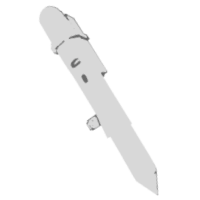
\includegraphics[width=0.25\textwidth]{imagenes/LogoSmartPen.png} 
 \vspace{0.5cm}

% Title

{\Huge\bfseries Dispositivo para detección de escritura mediante Deep Learning en
un sistema empotrado\\
}
\noindent\rule[-1ex]{\textwidth}{3pt}\\[3.5ex]
{\large\bfseries SmartPen\\[4cm]}
\end{minipage}

\vspace{2.5cm}
\noindent\hspace*{\centeroffset}\begin{minipage}{\textwidth}
\centering

\textbf{Autor}\\ {Antonio Priego Raya}\\[2.5ex]
\textbf{Directores}\\
{Juan José Escobar Pérez\\
Jesús González Peñalver}\\[2cm]
%
\includegraphics[width=0.15\textwidth]{imagenes/tstc.png}\\[0.1cm]
%\textsc{Departamento de Teoría de la Señal, Telemática y Comunicaciones}\\
%\textsc{---}\\
%Granada, mes de 201
\end{minipage}
%\addtolength{\textwidth}{\centeroffset}
\vspace{\stretch{2}}

 
\end{titlepage}





\cleardoublepage
\thispagestyle{empty}

\begin{center}
{\large\bfseries Detección de escritura mediante Deep Learning en
un sistema empotrado\\
}
\textsc{---}\\
{\small\bfseries SmartPen}\\
\end{center}
\begin{center}
Antonio Priego Raya\\
\end{center}

%\vspace{0.7cm}
\noindent{\textbf{Palabras clave}: TinyML, Machine learning, Deep learning,
Sistemas empotrados, Reconocimiento letras, Redes neuronales convolucionales
...}\\

\vspace{0.7cm}
\noindent{\textbf{Resumen}}\\

Creación de un dispositivo autónomo con forma de lápiz en el que integrar un
sistema empotrado, concretamente se hará uso de la \textit{Arduino Nano Sense 33 BLE}.
El propósito de este dispositivo será la detección de letras en tiempo
real, registrando el movimiento del dispositivo y rasterizando el mismo
para procesarlo y clasificarlo.

Para este procesamiento y clasificación de las letras registradas, se empleará
\textit{deep learning}, concretamente un modelo de red neuronal convolucional. Con la
particularidad de ejecutar el procesamiento del modelo en el propio
dispositivo, para dotarlo de autonomía.

Esta autonomía está complementada por una batería que garantiza su independencia.
Por tanto se desarrollarán todos los pasos propios del trabajo con
redes neuronales: diseño del modelo, recolección de datos, entrenamiento
del modelo, su testeo, etc.

Complementario al dispositivo, también se creará un interfaz de usuario donde acceder
a las funciones que se desarrollen para este dispositivo.
\cleardoublepage


\thispagestyle{empty}

\begin{center}
       {\large\bfseries Deep Learning handwriting detection in an embedded system\\
       }
       \textsc{---}\\
       {\small\bfseries SmartPen}\\
       \end{center}
       \begin{center}
       Antonio Priego Raya\\
\end{center}

%\vspace{0.7cm}
\noindent{\textbf{Keywords}: TinyML, Machine learning, Deep learning,
Embedded systems, Letter detection, Convolutional neural networks ....}\\

\vspace{0.7cm}
\noindent{\textbf{Abstract}}\\

Creation of an autonomous device in the shape of a pencil in which to integrate
an embedded system, specifically using the Arduino Nano Sense 33 BLE.
The purpose of this device is to detect letters in real time,
recording the movement of the device and rasterizing it to be processed and classified.

A Deep Learning model will be used for this letter processing and classification,
specifically a convolutional neural network model.
With the
particularity of executing the processing of the model in the device itself,
in order to provide it with autonomy.

This autonomy is complemented using a battery that guarantees its independence.
Therefore, all the steps involved in working with neural networks will be developed:
design of the model, data collection, model training, testing, etc.

Complementary to the device, a user interface will also be created to access the
functions developed for this device.

\chapter*{}
\thispagestyle{empty}

\noindent\rule[-1ex]{\textwidth}{2pt}\\[4.5ex]

Yo, \textbf{Antonio Priego Raya}, alumno de la titulación \textit{Grado en Ingeniería Informática}
de la \textbf{Escuela Técnica Superior
de Ingenierías Informática y de Telecomunicación de la Universidad de Granada}, con DNI 31033948W, autorizo la
ubicación de la siguiente copia de mi Trabajo Fin de Grado en la biblioteca del centro para que pueda ser
consultada por las personas que lo deseen.

\vspace{6cm}

\noindent Fdo: Antonio Priego Raya

\vspace{2cm}

\begin{flushright}
Granada a 8 de Julio de 2022
\end{flushright}


\chapter*{}
\thispagestyle{empty}

\noindent\rule[-1ex]{\textwidth}{2pt}\\[4.5ex]

D. \textbf{Jesús González Peñalver}, Catedrático del departamento de Arquitectura y Tecnología de Computadores de la Universidad de Granada.

\vspace{0.5cm}

D. \textbf{Juan José Escobar Pérez}, Profesor Sustituto Interino del departamento de Arquitectura y Tecnología de Computadores de la Universidad de Granada.

\vspace{0.5cm}

\textbf{Informan:}

\vspace{0.5cm}

Que el presente trabajo, titulado \textit{\textbf{Dispositivo para detección de escritura mediante Deep Learning en
un sistema empotrado}},
ha sido realizado bajo su supervisión por \textbf{Antonio Priego Raya}, y autorizamos la defensa de dicho trabajo ante el tribunal
que corresponda.

\vspace{0.5cm}

Y para que conste, expiden y firman el presente informe en Granada a X de mes Julio de 2022.

\vspace{1cm}

\textbf{Los directores:}

\vspace{5cm}

\noindent \textbf{Jesús González Peñalver \ \ \ \ \ \ \ \ \ \ \ Juan José Escobar Pérez}

\chapter*{Agradecimientos}
\thispagestyle{empty}

       \vspace{1cm}


Poner aquí agradecimientos...

